%%%%%%%%%%%%%%%%%%%%%%%%%%%%%%%%%%%%%%%%%%%%%%%%%%%
% DOCUMENT CLASS DECLARATION
%%%%%%%%%%%%%%%%%%%%%%%%%%%%%%%%%%%%%%%%%%%%%%%%%%%
%% Use the following options:
% \documentclass[paper type% ("letterpaper" required)
% , one or two sided% ("oneside" or "twoside")%
% , font size% ("12pt" required)%
% , document type% ("these", "memoire", "memoirepararticles", "memoireprojet" or "thesepararticles")%
% , document language ("francais" or "english)%
% , addition options% ("creativecommons" if the document is under the creative commons license, "hyperref", "withAlgo2e" to use algorithm2e package with proper formating)
%]{thETS}

%\newtheorem{remark}{Remark}[section]
%%%%%%%%%%%%%%%%%%%%%%%




%% Exemple with a Ph.D thesis under creative commons, using hyperref
\documentclass[letterpaper%
, twoside%
, 12pt%
,memoire%
, english%
,creativecommons,hyperref, withAlgo2e %
]{thETS}


\usepackage{algorithm}
\usepackage{algpseudocode}

\numberwithin{algorithm}{chapter}

\usepackage{makecell}
\usepackage{amsmath}
\usepackage{graphicx}
\usepackage{array}



\usepackage{tikz}
\def\checkmark{\tikz\fill[scale=0.4](0,.35) -- (.25,0) -- (1,.7) -- (.25,.15) -- cycle;} 

%%%%%%%%%%%%%%%%%%%%%%%%%%%%%%%%%%%%%%%%%%%%%%%%%%%
% IMPORTANT: PRINTING WITH THE PROPER MARGINS
%%%%%%%%%%%%%%%%%%%%%%%%%%%%%%%%%%%%%%%%%%%%%%%%%%%
%% Always set the "scaling" option to "none" in the prining options 
%% to print the generated PDF with the proper margins.
%%%%%%%%%%%%%%%%%%%%%%%%%%%%%%%%%%%%%%%%%%%%%%%%%%%


%%%%%%%%%%%%%%%%%%%%%%%%%%%%%%%%%%%%%%%%%%%%%%%%%%%
% DECLARATION OF AN ADDITION LIST OF REFERENCES
%%%%%%%%%%%%%%%%%%%%%%%%%%%%%%%%%%%%%%%%%%%%%%%%%%%
%% Exemple of an additional list of references called "refs"
% "refs" is used as a suffix to all bibliography related commands
\newcites{refs}{LIST OF REFERENCES}

%%%%%%%%%%%%%%%%%%%%%%%%%%%%%%%%%%%%%%%%%%%%%%%%%%%
% TITLE PAGE OPTIONS
%%%%%%%%%%%%%%%%%%%%%%%%%%%%%%%%%%%%%%%%%%%%%%%%%%%
 -%%


\begin{document}

\pagenumbering{Roman}


\tableofcontents


%%- List of tables -%%
\listoftables


%%- List of figures -%%
\listoffigures

\listofalgorithms



 
\chapter{Methodology}

In this chapter I present my  architecture as well as the optimization model for GAN, called OGAN. First I present the system model and four components of my  architecture as in Figure \ref{fig:Model}, Small Base Station, Macro Base Station. 










\section{System Model}\label{sec:Model}




Due to the high cost, geographic deployment challenges, and the need for system agility, it is impractical to forward the backhaul traffic of every SBS via dedicated broadband Internet or fiber links, particularly in urban environments. I assume that the backhaul traffic of SBSs is forwarded to the core network through a shared wireless link between the SBSs and a MBS. Both the MBS and SBS can independently transmit user data and management data to their associated users. Although users can hand over between SBSs within macrocells, for simplification, I assume that during each wireless episode, users are served by a single SBS. For efficiency, the gateway is configured at the MBS, which typically has sufficient space to install massive antennas to receive the wireless backhaul traffic from SBSs. However, the capacity of the backhaul network remains a bottleneck, potentially limiting the densification of small cells in 5G UDNs (\cite{ge20165g}).


\begin{figure}[t]
    \centering
    \fbox{
        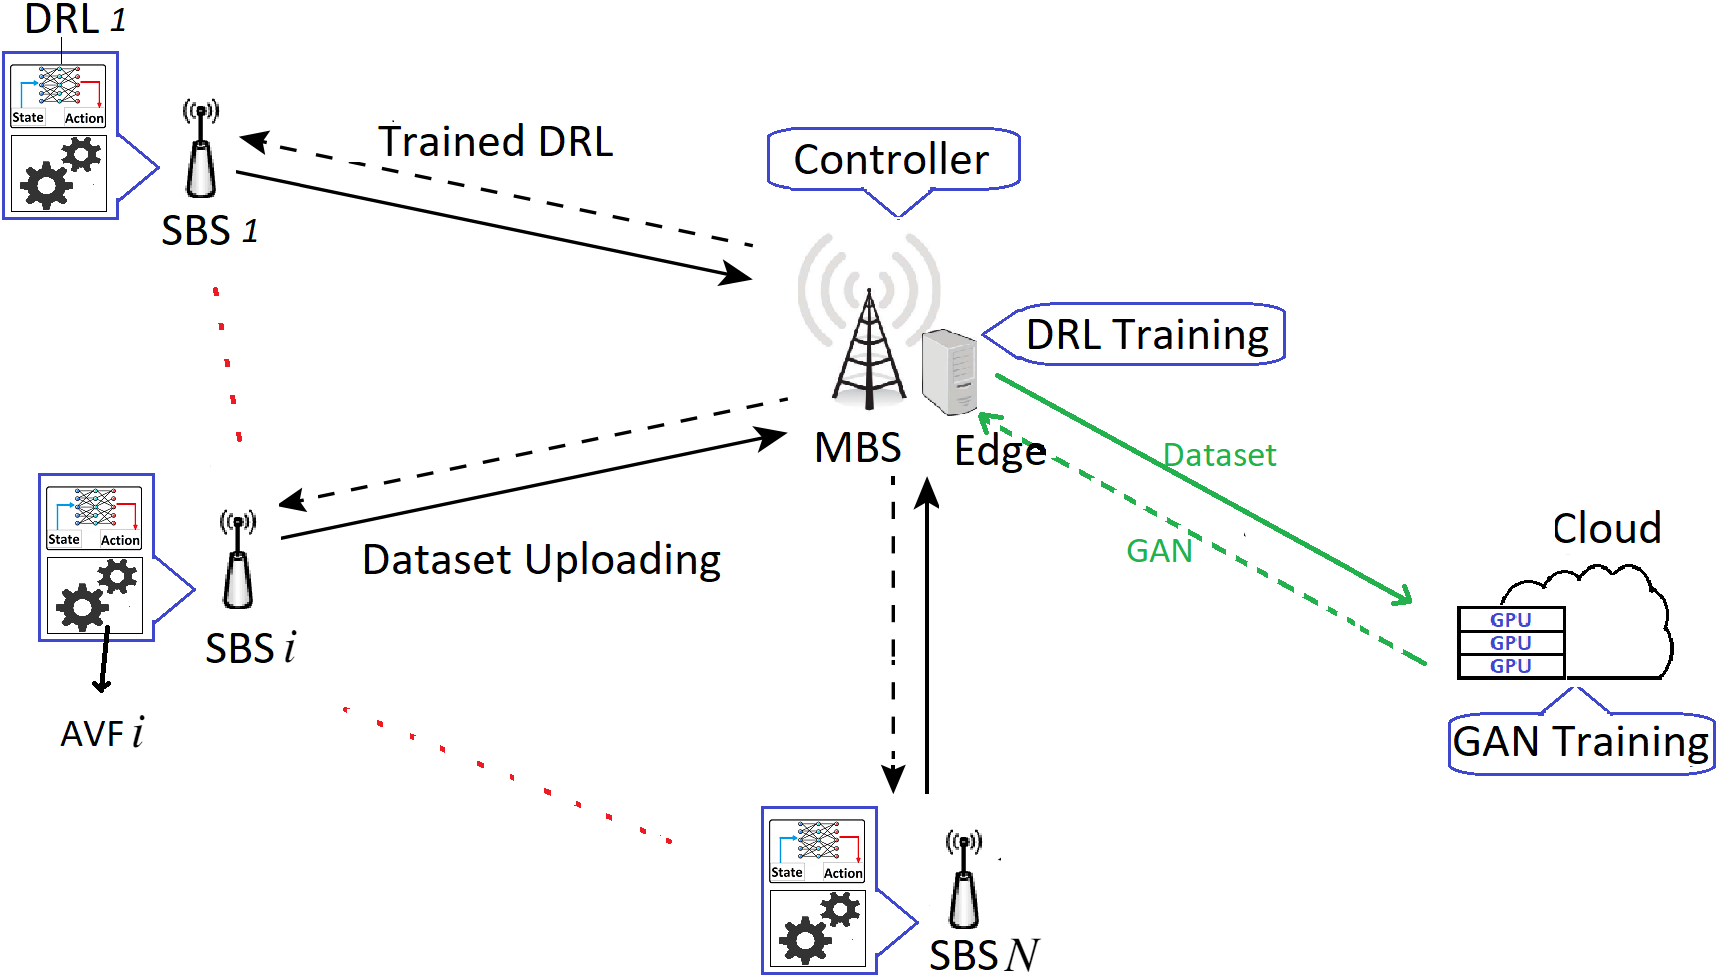
\includegraphics[width=0.95\textwidth]{5g dense- from FL-2 (2).png}
    }
    \\ \parbox{0.9\textwidth}{\caption[System Model]{System Model. A 5G UDN with a single MBS and $N$ SBSs. The architecture shows the workflow for training DRL models at the edge and GANs in the cloud. SBSs collect and upload GAN training datasets to the MBS, which then forwards them to cloud.}\label{fig:Model}}
\end{figure}




 The downlink channel of each SBS is shared based on OFDMA to deliver URLLC service. UDN network serves a set $\mathcal{L}$ of $L$ users distributed evenly among all SBSs. For simplicity, I assume each user $l$ is only served with a single SBS $i$, $\forall i \in \mathcal{N}$ and $\forall l \in \mathcal{L}$. The downlink transmission rate from the SBS $i$ to user \(l\) is given by:
\begin{equation}
 r_{l}(t) = \sum_{z=1}^{K_i} \rho_{lz}(t) B \log_{2} \left(1 + \frac{p_{lz}(t)h_{lz}(t)}{\sigma^2} \right), 
\end{equation}
where \(B\) is the bandwidth of the resource block (RB), and \(h_{ilz}(t)\) represents the time-varying channel gain of the transmission from the SBS $i$ to user \(l\) on RB \(z\) at time slot \(t\). \(p_{ilz}(t)\) denotes the downlink transmission power of the BS $i$ on RB \(z\) to user \(l\) at slot \(t\). $K_i$ is the number of RBs of SBS $i$ while \( \rho_{lz}(t) \) serves as the RB allocation indicator, with \( \rho_{ilz}(t) = 1 \) when RB \(z\) is allocated to user $l$ from SBS $i$. OFDMA resource allocation is performed distributed on each SBSs $i$ with its dedicated DRL agent, DRL $i$ where $i \in \mathcal{N}$. Following I present formulation of the DRL agent.


\subsection{Deep Reinforcement Learning}  I consider the DRL model presented in (\cite{kasgari2020experienced}) for 5G URLLC OFDMA resource allocation, as shown in Figure \ref{fig:enter-label}. At each transmission interval, DRL $i$ receives the current environment state and reward from the SBS $i$ as input. The DRL model incorporates two inputs as its reward to evaluate its performance and update its DNN parameters in each time slot: the total downlink power of SBS $i$ denoted as \( P_i(t) = \sum_{l} \sum_{z} p_{lz}(t) \), and the measured reliability of each user at each time slot t is ($1-\gamma_l(t)$) where $\gamma_l(t)$ is given by:
\begin{equation}
    \gamma_l(t) \approx 1 - \frac{\mu^{'}_l(t)}{\mu_l(t)},
\end{equation}
 where \( \mu^{'}_{l}(t) \) represents the number of packets received by user $l$ and \( \mu_l(t) \) is the total number of packets transmitted to user $l$ at time slot $t$. Note that it is an empirical measurement for unreliability so there is no requirements for assumptions about unreliability. 

The channel gains of each user, denoted by \(h_{lz}(t)\), the number of packets \( \hat{\mu}_l(t) \) transmitted to each user \(l\), and the average packet length \( \hat{\beta}_l(t) \) for each user \(l\) are the environment state of agent, formulated as \( s_t = (\hat{\mu}_l(t), \hat{\beta}_l(t),h_{lz}(t)) \) for all \(l \in L\), \(z \in K\). 


 Using these parameters as the state space, the DRL agent learns optimal policies for OFDMA resource allocation. To do that, DRL $i$ determines \( \rho_{lz}(t) \) and \( p_{lz}(t) \), its action, for all users served by SBS $i$. Through iterative assignment of \( \rho_{lz}(t) \) and \( p_{lz}(t) \) and receiving feedback across multiple time slots, the system can consistently uphold user reliability, latency, and throughput. The action \(a_t = (p_{lz}(t), \rho_{lz}(t))\) for all users \(l\) and RBs \(z\) which are  the transmission power and RB allocation to users. Subsequently, the reward of DRL is determined to  to ensure the QoS for URLLC.


\begin{figure}
    \centering
    \fbox{
        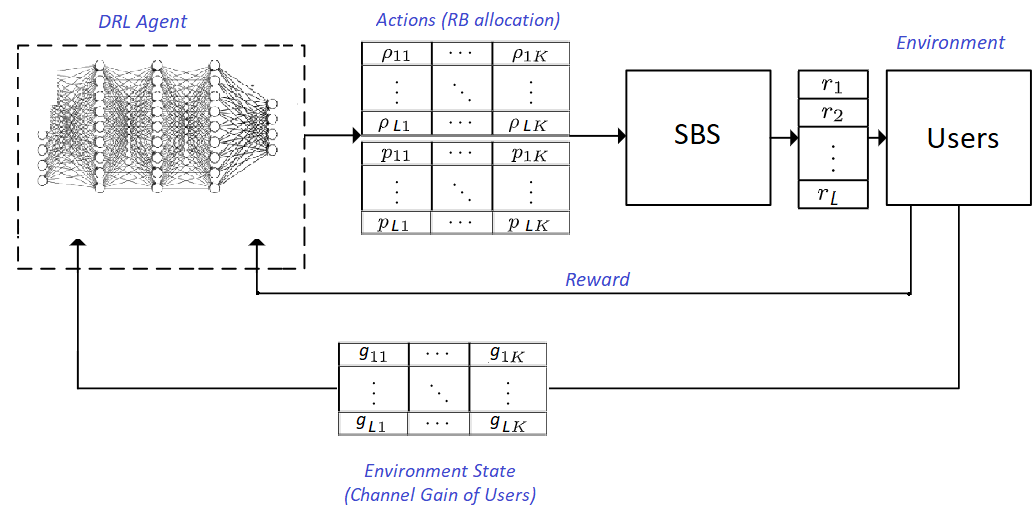
\includegraphics[width=0.95\textwidth]{Single_DRL_model.png}
    }
    \\ \parbox{0.88\textwidth}{\caption[DRL model for OFDMA RB allocation]{DRL model for OFDMA resource block (RB) allocation in a cell with \(L\) users and \(K\) sub-carriers. The DRL agent takes the environment state (Channel Gain Matrix of users) and outputs actions in the form of RB allocation matrices. These actions are then used by the SBS to determine the transmission rate of users. The reward is fed back to the DRL agent to update its policy and improve future allocations.}\label{fig:enter-label}}
\end{figure}








 
 Since SBSs have different characteristics, such as channel distributions, traffic patterns (\cite{zhang2021dual}), it is not feasible to implement a single DRL model for all SBSs. Therefore, each DRL $i$ is trained based on the dataset gathered from SBS $i$ to improve their performance. Although it is possible to train a single larger DRL model to be used for all SBSs, it increases the DNN size of DRL agents since they should learn data distribution of all of SBSs. By increasing DNN size, the training and inference time of DRL as well as computation and energy consumption of SBSs to take actions is increased. I then use a smaller DNN models for DRL and train a dedicated DRL based on dataset gathered from its SBSs. This way, with smaller DRL models, less computation is required for inference of DRL model that decreases the size, price and battery usage of SBSs.


  
  I consider a dynamic network scenario where changes occur slowly over time and are divided into episodes. I assume in each episode, the channel and traffic distribution of SBSs remain constant, as in (\cite{sun2022learning}). For SBS $i$, the remaining time till the end of the current episode is given as $T_i^{max}$. Episode time is based on application and other parameters which affect the channel distribution. Following I propose some approaches to estimate the value of $T_i^{max}$.


In the industrial environment, numerous factors can significantly impact channel distribution. Even slight alterations in these factors can be seen as significant channel distribution shifts. Challenges stemming from dust, temperature fluctuations, vibrations, humidity levels, object trajectories, materials, obstacles, and lighting are more pronounced in industrial settings compared to other environments. Additionally, signal interference from wireless devices and motors further complicates wireless communication in such environments. Given that many of these factors are linked to industrial processes, one approach to determining $T_i^{max}$ is to forecast it based on the factory's production schedule, taking the time of process changes as $T_i^{max}$ (\cite{li2017review}).

  In open spaces, weather forecasts can be utilized to predict variables such as temperature, humidity, precipitation, and sunlight, aiding in the determination of $T_i^{max}$. Similarly, in urban environments, in addition to the aforementioned factors, analyzing traffic patterns can provide valuable insights for predicting $T_i^{max}$.


Another general approach to determining $T_i^{max}$ involves prediction methods that estimate the number of active users or cell traffic load (\cite{wang2022spatial}). Sudden changes in these factors can alter the state-space distribution of DRL, potentially leading to the conclusion of the current wireless episode.

 Additionally, another way for UDNs to predict $T_i^{max}$ is by forecasting SBS on/off patterns (\cite{zhu2021joint}). In UDNs, frequency reuse indicates the level of interference from neighboring cells. When an SBS is toggled on or off, it affects the interference level of adjacent cells, thereby altering the channel distribution, which constitutes the state-space of a cell. Therefore, predicting the on/off status of cells can serve as $T_i^{max}$ for other adjacent cells using the same frequencies.




\subsection{GAN model}

The presence of rare samples within the state-space of DRL can lead to unreliable URLLC service. To mitigate this issue, I train a GAN with rare samples to augment the training datasets for each DRL. Given my  assumption that the state-space distributions of DRLs from different SBSs are dissimilar, it follows that the distributions of their rare samples also differ. Consequently, I propose for training a dedicated GAN for each SBS, which reduces the time and computational resources required for training. Training multiple smaller GANs consumes less time and allows for parallel training across multiple GPUs, thereby enhancing training speed. Subsequently, each GAN is utilized to augment the training dataset for its corresponding DRL. Therefore, for each SBS $i$, I propose training a GAN, denoted as GAN $i$. The training dataset for GAN $i$ comprises rare samples collected from SBS $i$, enabling more effective augmentation of the training datasets for DRL $i$.




\subsection{GAN}
In this section I present the GAN model used for augmenting rare smaples. My GAN has two DNNs, a Generator and a Discriminator, which are trained concurrently through adversarial processes. The architecture and functionality of each component are detailed below.


\subsubsection{Discriminator}


The Discriminator is a convolutional neural network that classifies input (OFDMA channel gain matrix) as real or generated (fake). Its output is a single scalar value indicating the probability that the input is real. The Discriminator network structure includes:

\begin{enumerate}
    \item \textbf{Convolutional Layers}: The Discriminator consists of five convolutional layers. The first layer takes a single-channel input image and applies a convolutional filter to produce feature maps. Subsequent layers increase the number of feature maps while reducing the spatial dimensions, allowing the network to capture increasingly abstract features.
   

\item  \textbf{Activation Functions}: Leaky ReLU activations with a negative slope of 0.2 are used after each convolutional layer, except the final layer, where a sigmoid function is applied to produce a binary classification output.
\end{enumerate}


\subsubsection{Generator}



The Generator is a deconvolutional neural network (also known as a transposed convolutional network) that synthesizes fake samples (channel gain matrix) from random noise vectors. The architecture of the Generator includes:

\begin{enumerate}
    \item \textbf{Transposed Convolutional Layers}: The Generator consists of five transposed convolutional layers. These layers progressively upsample the input noise vector to produce a high-resolution output. The first layer transforms a 100-dimensional noise vector into feature maps with depth '8D' and applies batch normalization. The final (fifth) layer outputs a single-channel matrix with parameter values in the range \([-1, 1]\).
    \item \textbf{Activation Functions}: ReLU activation is used after each transposed convolutional layer except the final layer, where a tanh function is applied to ensure the output image has pixel values in the desired range.
\end{enumerate}






\subsubsection{Training Procedure}

The training process involves alternating updates to the Generator and the Discriminator:

\begin{itemize}
    \item \textbf{Discriminator Training}: The Discriminator is trained to maximize the probability of correctly classifying real samples and minimize the probability of incorrectly classifying generated samples.
    \item \textbf{Generator Training}: The Generator is trained to minimize the probability of the Discriminator correctly identifying generated fake samples, effectively maximizing the Discriminator's error rate.
\end{itemize}

The overall objective is to reach a Nash equilibrium where the Discriminator cannot distinguish between real and generated samples better than random chance, thus ensuring the Generator produces highly realistic (rare) samples.



%(put GAN model here)


\subsection{Architecture for training GAN/DRL in UDN}

In this section I explain my  architecture for optimal resource allocation for training GAN and DRL in resource limited 5G UDNs. My proposed architecture is consisted of four main elements, small base station (SBS), macro base station (MBS), mobile edge computing (MEC) and cloud. 




Due to the computational limitations of SBSs, DRL models and GANs are trained on a Mobile Edge Computing (MEC) server associated with the MBS or on the cloud data center. SBSs often lack the processing power and memory required for intensive training tasks, which necessitates offloading these tasks to more capable servers.

Training GANs, in particular, is computationally intensive due to their DNNs with a large number of parameters, resulting significantly longer training times when using CPU servers. In contrast, training DRLs in a simulator, although less demanding than GANs, still require substantial computational resources, mostly CPUs since simulator environment demands more CPU powers. If the training time exceeds a predefined maximum duration, wireless episode (\(T_i^{max}\)) in my  case, both the GAN and DRL models can become outdated. This is because the environment's dynamics and the data distribution used for training these models may change significantly after \(T_i^{max}\), rendering the models less effective or even obsolete.

To address these issues, my  architecture proposes offloading training GANs in the cloud, where powerful GPUs are optimized for accelerating the training process of GANs. This setup significantly reduces the training time, ensuring that the models are updated before \(T_i^{max}\) is reached. The cloud infrastructure also provides scalable resources, allowing for the training of larger and more complex models as needed.

Additionally, the MEC server plays a crucial role in maintaining the performance of DRL models. By offloading the less computationally demanding DRL training tasks to the MEC server, we can achieve a balance between latency and computational efficiency. This setup enables real-time decision-making for the SBSs while still benefiting from the robust training capabilities of the cloud for GANs.

In summary, my  architecture leverages the strengths of both MEC servers and cloud data centers to address the computational challenges of training DRLs and GANs. By strategically offloading tasks based on their computational requirements, we ensure timely updates and maintain the effectiveness of the models in dynamic environments.





 
 
  
Another rationale for training GANs in the cloud is the relatively smaller dataset size required for GAN training compared to training DRL models. In my  problem, GANs typically utilize datasets consisting of only a few thousand samples, whereas DRL models require datasets with tens of thousands of samples. Consequently, training GANs in the cloud generates less traffic on the connection link between MBS and the cloud infrastructure compared to training DRL models in the cloud. By offloading GAN training to the cloud, I minimize the burden on the connection link, ensuring efficient data transfer without overwhelming the network. 
  

  On the other hand, I use servers with CPUs on edge for training DRLs. Since training DRL with real data samples gathered from cells causes traffic challenge, we have to store those datasets on MEC and use MEC resources to train DRLs. It has two other benefits also: Firstly, as mentioned before DRLs model used for OFDMA resource allocation is much smaller than GAN model. So its training on CPU servers take less time compared to training GAN on the same server. Moreover, during training of DRL in a simulator, more demands CPU resources than GPUs. 


On the contrary, we employ servers equipped with CPUs at MEC for training DRL models. Training DRL models with real data samples collected from SBSs presents a traffic challenge, necessitating the storage of these datasets on MEC platforms. By utilizing MEC resources for DRL training, we not only mitigate traffic challenges but also capitalize on two additional benefits. Firstly, as previously mentioned, DRL models utilized for Orthogonal Frequency Division Multiple Access (OFDMA) resource allocation are significantly smaller compared to GAN models. Consequently, their training on CPU servers consumes less time in comparison to training GANs on the same server. Furthermore, during the training of DRL models in a simulator, there is a higher demand for CPU resources than for GPUs. By leveraging CPU resources at the edge for DRL training, I optimize computational efficiency while also addressing traffic challenges associated with real data sample usage. This approach ensures timely and effective training of DRL models, facilitating their deployment in communication systems with minimal disruption.




Following I present the detail of four components of my  architecture which is controlled with a central controller.


\subsubsection{Small Base Station}

Here, I will explain the first element of my  architecture. The main responsibility of the SBS is to provide URLLC service to users within its coverage area. It employs a DRL agent for optimal OFDMA resource allocation. Another responsibility of the SBS is to collect datasets for training DRL and GANs, sending these datasets via the backhaul to the MEC or cloud through the MBS. Additionally, the SBS has an AVF agent, discussed in the next section, to collect and store rare samples from the environment for GAN training. As previously mentioned, to remain cost-efficient, SBSs have limited computational power, insufficient for training DNNs. Therefore, the training of DRL and GANs should be conducted on the MEC and/or cloud. 

Following this, I will provide a more detailed explanation of the components of the SBSs.

\subsubsection{Finding Rare Samples}

To detect rare state-spaces, I utilize a failure probability predictor known as AVF (\cite{uesato*2018rigorous}). The primary role of the AVF agent is to identify failure situations encountered by a DRL agent. Typically, Monte Carlo simulations are employed to find failure situations and estimate their probabilities by comprehensively testing various conditions. However, AVF leverages data already collected during the training and implementation processes, eliminating the need for extensive Monte Carlo simulations to identify failure conditions. This approach streamlines the identification of rare state-spaces and enhances the efficiency of failure detection in DRL systems.

Given that packet loss significantly impacts URLLC reliability, I designate it as a critical failure scenario for my  AVF model. The objective of AVF is to find cases where the DRL agent may fail to provide reliable communication. The episode duration for AVF is determined by \( \min(d_0, ..., d_i, ..., d_N) \), where \( d_i \) represents the URLLC transmission delay of SBS \( i \). In each SBS \( i \), an AVF agent, AVF \( i \), continuously monitors the DRL agent's performance to identify failure cases to be used as rare samples. The AVF agent then maintains a dataset \( \Upsilon_i \), which contains these rare samples for training GAN \( i \).

The dataset \( \Upsilon_i \) accommodates \( N_{\Upsilon_i} \) samples, capturing instances of failure scenarios. When \( \Upsilon_i \) reaches its capacity or when a wireless episode transitions, the oldest samples are replaced by the most recent ones. This ensures that the dataset remains up-to-date and relevant, continuously providing valuable data for training GANs to improve system robustness.





%(add a figure of the agent and how it works)




\subsubsection{Generative Adversarial Network} 

During the training of a GAN, its discriminator (Di) evaluates the quality of the generated samples produced by the generator (Ge) using feedback measures known as Neural Net Distance (NND). NND quantifies the degree of dissimilarity between the generated data and the real dataset. Various metrics can be employed as NND during the training of GANs. The training process involves solving a minimax problem through empirical risk minimization, wherein an estimation error \(\epsilon\) is associated with NND. Estimation error \(\epsilon\) refers to the difference between the empirical risk (i.e., the average loss over the training data) and the true risk (i.e., the expected loss over the entire data distribution).


Based on the analysis of Rademacher complexity conducted by the authors in (\cite{ji2021understanding}), they identify an upper bound error associated with NND, denoted as $E$. It's noteworthy that their investigation focuses on GAN models employing Rectified Linear Unit (ReLU) activation functions. In their proposed model, they consider the size of the training dataset, denoted as $N_\Upsilon$, and the number of unique fake samples, denoted as $m$, generated and evaluated during the training phase. Particularly, when the dimension of the input noise vector is large, such as 128, the parameter $m$ can be regarded as the number of training iterations for the GAN model. Inspired by their research, I suggest a compressed version of $E$ as follows:
\begin{equation}\label{eq:gan_error}
E = \frac{V}{\sqrt{m}} + \frac{W}{\sqrt{N_\Upsilon}},
\end{equation}
where $V$ and $W$ are sums of the Frobenius norm of the generator and discriminator parameter matrices, respectively. When $E$ reduces, GAN's probability distribution of the generated data samples approaches the probability distribution of real data. Note that Eq. \ref{eq:gan_error} indicates that by increasing the values of $m$ (number of GAN training iterations) and $N_\Upsilon$ (number of training samples), the value of $E$ decreases. This observation implies that as more training iterations and samples are utilized, the upper bound error associated with NND in GAN models diminishes.

According to (\cite{zhou2020learning}), $V$ and $W$ can be obtained through offline training of GANs using different sample size $N_{\Upsilon}$. The sizes of my  datasets used for offline training are selected from the list ($N_{\Upsilon}^{(1)}, N_{\Upsilon}^{(2)}, N_{\Upsilon}^{(3)}, N_{\Upsilon}^{(4)})$ = (1,000, 2,000, 3,000, 4,000). After conducting 500 GANs trials for each values of ${N_{\Upsilon}}$, I calculate the averaged values for $V$ and $W$, labeled as $\bar{V}_{N_{\Upsilon}}$ and $\bar{W}_{N_{\Upsilon}}$, respectively. The resulting tuples of \{$\bar{V}_{N_{\Upsilon}}$, ̄$\bar{W}_{N_{\Upsilon}}$\} corresponding to the aforementioned list are given by (\{14.41, 13.17\}, \{15.2, 14.1\}, \{14.80,13.78\}, \{14.52, 13.42\}). 


\begin{table}[h]
\centering
\caption{Offline Training Results}
\label{tab:offline_training}
\begin{tabular}{|c|c|c|}
\hline
\textbf{$N_{\Upsilon}$} & \textbf{$\bar{V}_{N_{\Upsilon}}$} & \textbf{$\bar{W}_{N_{\Upsilon}}$} \\ \hline
1,000 & 14.41 & 13.17 \\ \hline
2,000 & 15.2 & 14.1 \\ \hline
3,000 & 14.80 & 13.78 \\ \hline
4,000 & 14.52 & 13.42 \\ \hline
\end{tabular}
\end{table}



Resolving the critical challenges of mode collapse and divergence in GAN training typically demands larger datasets (\cite{bang2021mggan}). In my  case, a minimum of 1,000 samples is required to train GANs to achieve the acceptable quality, based on my  experimental findings. When the dataset is large and complex, training GANs in resource limited environments, is more challenging since in high dimensional sample spaces, GANs struggles to cover all modes. Hence, for each SBS, I train multiple smaller GANs to exploit the temporal correlations among data samples collected in close proximity. This strategy not only reduces the training time and memory requirements of GANs, but also reduces the risk of mode collapse and training divergence.



\subsubsection{Cloud Datacenter}

 As mentioned before, in 5G URLLC environments, the dataset distribution (environment) changes more frequently, with shifts may occur on the order of minutes. As a result, the frequency of GAN training must be higher, and the training deadlines are tighter. To reduce training time, it is required to train them in powerful GPUs provided by cloud datacnters. Furthermore, I train multiple smaller GANs (one for each SBS) rather than a single larger GAN shared among all SBSs. This strategy reduces the dataset size significantly compared to training large GANs for high-quality image or video generation. Consequently, the transmission time required for sending the dataset to the cloud is reduced, enabling us to leverage the higher processing power of GPUs available in the cloud, rather than relying on weaker MEC servers. 
 
 
 The cloud datacenter is equipped with $N_g$ GPUs, each operating at a frequency of $F_g$. For simplicity, I assume that each GAN is trained on a single GPU, and GPUs are only released once the training task for their respective GAN is completed. This straightforward setup simplifies the resource allocation process and ensures that each GPU is fully dedicated to the training of its assigned GAN until completion. SBSs upload their datasets, denoted as $\Upsilon_i$, to the cloud through the MBS. The training time of GAN $i$ is given by $T_{i}^{gan} = m_i.\eta_i^{(g)}/F_g$, where $m_i$ is the number of training steps for GAN $i$ ($\mathbf{m} = \{m_i\}$), $\eta_i^{(g)}$ denotes the required GPU cycles for GAN $i$, and $F_g$ is the processing capacity of the GPU. Finally, the trained GANs are transmitted back to the MEC platform for dataset augmentation.



\subsubsection{Mobile Edge Computing (MEC)}

The large datasets used for DRL fine-tuning should be hosted in the MEC to reduce data transmission overhead to the cloud. Since training a DRL requires very large datasets, in my  architecture I propose to train DRLs in the MEC to decrease the overhead of sending these datasets to the cloud. I assume that a dataset from the current episode is available in the MEC. Each time we train a new GAN, we add the augmented dataset from the GAN to this existing dataset. 



The MEC has $N_c$ CPU cores in total, each operating at a frequency of $F_c$ GHz. The pre-training time for DRL $i$ is given by $T_{i}^{tr} = (\Phi_i.\eta_i^{(c)})/(F_c . c_{i})$, where $c_i$ is the allocated number of CPU cores, and $\Phi_i$ is the number of steps to train DRL $i$. I denote the vector $\mathbf{c} = \{c_i\} \in \mathbb{R}^N$. A maximum of $\Psi_i$ CPU cores can be used for training DRL $i$. Since the data distribution remains constant within an episode, the number of training iterations for DRL agent $i$, denoted as $\Phi_i$, is estimated based on the number of training iterations of its current version. As all DRL agents are pre-trained, $\Phi_i$ is readily available from the start.


 The time required for SBS $i$ to upload dataset $\Upsilon_i$ to MBS is $T_i^{com} = |\Upsilon_i| / R_i$ , where $|\Upsilon_i|$ is the size of $\Upsilon_i$ in MByte, and $R_i$ is the available bandwidth from SBS $i$ to the MBS given by $R_i = B_i . log_2(1+SNR_i)$ where $B_i$ is the channel bandwidth of SBS $i$ and $SNR_i$ is its average signal-to-noise ratio which is assumed to be constant over a long period of time (\cite{xie2023edge}). Besides, since the size of DNNs (GAN and DRL) is very small compared to the dataset, their transmission time can be discarded or be a small constant number in my  model.


\subsubsection{Central Controller}

%\begin{figure}
%    \centering
 %   \includegraphics[width=0.95\linewidth]{controller diagram.jpg}
  %  \caption{Enter Caption}
   % \label{fig:enter-label}
%\end{figure}



\begin{algorithm}[!h]

\caption{Controller Algorithm}

\label{alg:cnt}

\KwIn{inputs set:($\eta_i^{(g)}, \eta_j^{(c)}, E_i^{min}, \Psi_i, T_i^{max}, \Phi_i, B, B_i, N_\Upsilon, N_g, N_c, N, F_g, F_c$)} 
\KwOut{outputs set:($m_i, c_i, z_i$)}
\BlankLine

Monitor to detect changes in $N_g$ and $N_c$ 

\For{(all GPUs and CPUs)}{
    \If{(changes in $N_g$ or $N_c$ occur)}{
        \If{($N_g > 0$ and $N_c > 0$)}{
            \For{(all SBS $i \in \mathcal{N}$ ($i=1,...,N$))}{
            
                Pre-fetch \{$\nu_i^t$, $\nu_i^l$, $|\Upsilon_i|$, $B_i$\} 
                
                Calculate $\beta_i = \frac{\nu_i^l}{\nu_i^t}$ 
            }
            
            Solve OGAN 
            
            \For{(all SBS $i \in \mathcal{N}$ ($i=1,...,N$))}{
                \If{($z_i == 1$)}{
                    send $\mathbf{c}$ to MEC 
                    
                    send $\mathbf{m}$ to cloud 
                    
                    send $z_i$ to SBS $i$ to upload GAN training dataset 
                }
                Initiate GAN training 
                
                After GAN training completion, send every GAN $i$ to SBS $i$ 
                
                Initiate DRL training 
                
                Implement trained DRL $i$ on SBS $i$ 
            }
        } 
    }
}
return to the initial stage (line 1) 

\end{algorithm}

%(put more explanation about algorithm)


 The central controller located on the MBS, is responsible for monitoring and allocating system resources by prefetching commands from other components. Once a GPU or CPU core is released, the controller runs an optimization model named OGAN (see Section \ref{sec:ogan}), to schedule GAN and DRL training. OGAN determines the SBSs to train GANs as well as the optimal training steps $\mathbf{m}$ and computational resource $\mathbf{c}$. The controller's routine, as shown briefly in Algorithm 1, involves the following main steps:

\begin{enumerate}

    \item Continuously monitor both MEC and cloud to detect changes in available GPUs ($N_g$) and CPU cores ($N_c$). 
    \item If $N_g$ or $N_c$ changes and both of them are greater than zero, initiate pre-fetching of the following parameters from SBS $i$: $\nu_i^t$ (total transmitted packets), $\nu_i^l$ (total packet loss), $|\Upsilon_i|$ (dataset size), and $B_i$ (available back-haul bandwidth).
    \item Calculate a weight factor $\beta_i = \nu_i^l/\nu_i^t$ to assess the reliability of SBS $i$. For a fair comparison of SBSs based on their contribution to system unreliability, compute the normalized $\Tilde{\beta_i}$.
    \item  Solve OGAN to determine whether a GAN should be trained for SBS $i$ (variable $\mathbf{z}$), then allocates resources on cloud (variable $\mathbf{m}$) and MEC (variable $\mathbf{z}$) accordingly.
    
    \item If $\mathbf{z}$ == 0, return to the initial step, awaiting to change in $N_c$ and $N_g$.
    
    \item When the training is compeleted, send GAN generator DNNs to the MEC, where they are employed to augment the training datasets for their respective DRLs.
    
    \item Start training (fine-tuning) new DRLs at the MEC servers, and when they are completed, replace the existing ones with the newly trained ones.

\end{enumerate}

 Fine-tuning DRL $i$ is performed with $c_{i}$ CPU cores. Each time OGAN is called, it may dynamically adjust the number of cores assigned to a DRL during its training at the MEC, which might involve decreasing $c_i$ to increase $c_j$,  $\forall i,j \in \mathcal{N}$. As a result, this algorithm maximizes the efficiency of both cloud and MEC in order to train GAN and DRLs, ultimately resulting in higher quality and reliability for URLLC.  


Note that, since the number of SBSs exceeds the number of available GPUs, it is impossible to train all SBSs in one round. The maximum number of SBSs selected for training each time OGAN is called is equal to the number of GPUs, $N_g$. Whenever the training of a GAN model on a GPU is completed, or when the training of one of the DRL models finishes and CPU cores are released, OGAN is called again to determine resource allocation and assign resources for training the current GANs or choosing a new one.










\begin{table}[htp]
\centering
\caption{OGAN's input Parameters}
\label{tab:parameters}
\renewcommand{\arraystretch}{1.5} % Adjust this value to increase the height of all rows
\begin{tabular}{|c|l|}
\hline
\multicolumn{2}{|c|}{\textbf{Input Parameters}} \\
\hline
$\eta_i^{(g)}$ & The number of GPU cycles used in each iteration of GAN $i$ training \\
\hline
$\eta_j^{(c)}$ & The number of CPU cycles used for each step in pre-training DRL $i$ \\
\hline
$E_i^{min}$ & Lower bound of the estimation error for GAN $i$ \\
\hline
$\Psi_i$ & Maximum number of CPU cores can assigned for pre-training of DRL $i$ \\
\hline
$T_i^{max}$ & Remaining time until the end of current wireless episode \\
\hline
$\Phi_i$ & The upper bound of the training step for pre-training of DRL $i$ \\
\hline
$B$ & Shared bandwidth from SBS $i$ to MBS \\
\hline
$B_i$ & Bandwidth from SBS $i$ to MBS \\
\hline
$N_\Upsilon$ & Dataset storing rare samples of DRL $i$ \\
\hline
$N_g$ & The number of GPUs available in the cloud \\
\hline
$N_c$ & The number of CPU cores available in the edge \\
\hline
$N$ & Number of all SBSs \\
\hline
$F_g$ & Frequency of each GPU \\
\hline
$F_c$ & Frequency of each CPU \\
\hline
\end{tabular}
\end{table}




\section{Optimized GAN Training}\label{sec:ogan}






\subsection{Problem formulation}\label{prob_formulation}




 my  proposed resource-constrained GAN optimization model, OGAN is as follow:  





\begin{subequations} \label{eq:subeqnsss}
\begin{align}
& \min_{\mathbf{z}, \mathbf{m}, \mathbf{c}} \sum_{i=1}^{N}{\Tilde{\beta_i}((1-z_i)T_i^{max} + z_i(T_i^{com} + T_i^{gan} + T_i^{tr} + \alpha(\frac{\bar{V}_{N_\Upsilon}}{\sqrt{m_i}} + \frac{\bar{W}_{N_\Upsilon}}{\sqrt{N_\Upsilon_i}})))} \label{eq:obj} \\
\text{s.t.} & \nonumber \\
& z_i(T_{i}^{com} + \frac{m_i.\eta_i^{(g)}}{F_g} + \frac{\Phi_i.\eta_i^{(c)}}{F_c . c_{i}}) \leq T_{i}^{max} , \quad \forall i \in \mathcal{N},	\label{eq:time}\\
& z_i(\frac{\bar{V}_{N_\Upsilon}}{\sqrt{m_i}} + \frac{\bar{W}_{N_\Upsilon}}{\sqrt{N_\Upsilon_i}}) \leq E_i^{min} , \quad \forall i \in \mathcal{N}, \label{eq:error}\\
& \sum_{i=1}^{N}{z_i . R_i} \leq R, \label{eq:R_all} \\
& \sum_{i=1}^{N}{z_i . B_i} \leq B, \label{eq:bw_all} \\
& \sum_{i=1}^{N}{c_i} \leq N_c, \label{eq:sum_cpus} \\
& 0 \leq c_{i} \leq  \Psi_i , \quad \forall i \in \mathcal{N}, \label{eq:c_limits} \\
& \sum_{i=1}^{N}{z_i} \leq N_g, \label{eq:sum_gpus} \\
& 1 \leq m_{i}, \quad \forall i \in \mathcal{N}, \label{eq:min_m} \\
& z_i \in \{0,1\}, \quad \forall i \in \mathcal{N}. \label{eq:binary_z}
\end{align}
\end{subequations}



The objective function in (\ref{eq:obj}) minimizes two components. The first component, $(1-z_i)T_i^{max}$, represents the time DRL $i$ operates without fine-tuning its parameters using a GAN. In the case of $z_i=1$, the second component, $z_i(T_i^{com} + T_i^{gan} + T_i^{tr} + \alpha(\frac{\bar{V}_{N_\psilon}}{\sqrt{m_i}} + \frac{\bar{W}_{N_\epsilon}}{\sqrt{N_\epsilon_i}}))$, achieves a trade-off between two conflicting objectives: reducing $E_i$ and the total training time of GAN $i$ and DRL $i$, using the weight parameter $\alpha$. It is necessary to allocate a greater number of resources to training GAN $i$ when $\Tilde{\beta_i}$ is higher, as it indicates greater unreliability in communication with SBS $i$. Notably, more resources ($\mathbf{m}$, $\mathbf{c}$) reduce the training time (GAN, DRL), resulting in greater URLLC reliability.



Constraint (\ref{eq:time}) ensures the training time is within its allocated episode time. For a given $E_i^{min}$, constraint (\ref{eq:error}) guarantees that GAN $i$ undergoes a minimum number of training iterations, $m_i$, to prevent low-quality GANs. Bandwidth limit for uploading all of GAN training data from MBS to the cloud is indicated by constraint (\ref{eq:R_all}). Constraints (\ref{eq:bw_all}) limit the total available shared wireless backhaul bandwidth from SBSs to MBS.
Constraint (\ref{eq:sum_cpus}) limits the CPU usage of the MEC and each DRL. Constraint (\ref{eq:sum_gpus}) limits the number of GANs to the number of available GPUs and defines the minimum value of $m_i$. Since I assume a time-sharing policy for CPU cores, $c_i$ is a positive real number.



\begin{table}[t]
\centering
\caption{OGAN's decision variables}
\label{tab:parameters}
\renewcommand{\arraystretch}{1.5} % Adjust this value to increase the height of all rows
\begin{tabular}{|c|l|}
\hline

$m_i$ & Number of training iterations used for GAN $i$ \\
\hline
$c_i$ & Number of CPU cores allocated for pre-training DRL $i$ \\
\hline
$z_i$ & 1 if GAN $i$ is trained, 0 otherwise \\
\hline
\end{tabular}
\end{table}


\subsection{Solving OGAN}

The optimization problem associated with OGAN is inherently challenging due to its nature as a mixed-integer non-convex constrained optimization problem. Directly solving such a problem is computationally demanding and often infeasible. 

%%%%%%%%%%%%%%%%%%%%%%%%%%%%%%%%%%%%%%%%%%%%%%%%%%%
%  Appendix example:
%%%%%%%%%%%%%%%%%%%%%%%%%%%%%%%%%%%%%%%%%%%%%%%%%%%
%\appendix

%% To use more than one appendix
%\multiannexe

%% Appendix from an external file
% \include{extApp}



%%%%%%%%%%%%%%%%%%%%%%%%%%%%%%%%%%%%%%%%%%%%%%%%%%%
% BIBLIOGRAPHY AND REFERENCES
%%%%%%%%%%%%%%%%%%%%%%%%%%%%%%%%%%%%%%%%%%%%%%%%%%%

%%- Bibliography -%%
\cleardoublepage
% Single spacing for the bibliography
\begin{spacing}{1}
    \setlength{\bibsep}{\baselineskip}
    \setlength{\bibhang}{3em}
	\nocite{*} % The "nocite" command can be used to print references that haven't been used in the document. The "*" option specifies that every reference should be printed
	\bibliographystyle{bibETS} % ETS bibliography style
	\phantomsection % Adding an anchor for hyperref
	\addcontentsline{toc}{chapter}{BIBLIOGRAPHY} % Addition of the bibliography in the table of contents

	\bibliography{biblio_en} % List of bibliography files, biblio.bib is an example

\end{spacing}

%%- Other list of references, "refs" example --%
%%%%%%%%%%%%%%%%%%%%%%%%%%%%%%%%%%%%%%%%%%%%%%%%%%%
% IMPORTANT: HOW TO COMPILE AND PRINT ADDITIONAL REFERENCES (replace "refs" by the chosen name)
%%%%%%%%%%%%%%%%%%%%%%%%%%%%%%%%%%%%%%%%%%%%%%%%%%%
% Follow these three steps:
%   1. Compile the document once, to save the used references in refs.aux
%   2. Compile the references
% 		- On Linux: Use the "bibtex refs" command in the document folder
%		- On MacOSX (MacTex distribution): Use the "/usr/texbin/bibtex refs" command in the document folder
%		- On Windows: Edit the "update_refs.bat" script to put the right suffix ("refs" here), and launch the script
%   3. Recompile the document TWICE
%%%%%%%%%%%%%%%%%%%%%%%%%%%%%%%%%%%%%%%%%%%%%%%%%%%

%\cleardoublepage
% Same commands than for the bibliography, only with the "refs" suffix
\begin{spacing}{1}
    \setlength{\bibsep}{\baselineskip}
    \setlength{\bibhang}{3em}
	%\nociterefs{*}
	\bibliographystylerefs{bibETS}
	\phantomsection
%	\addcontentsline{toc}{chapter}{LIST OF REFERENCES}

%	\bibliographyrefs{refs}

\end{spacing}

\end{document}
